\documentclass[compress,handout,10pt]{beamer}
\usepackage{graphicx}
\newlength{\wideitemsep}
\setlength{\wideitemsep}{\itemsep}
\addtolength{\wideitemsep}{100pt}
\let\olditem\item
\renewcommand{\item}{\setlength{\itemsep}{0.5\baselineskip}\olditem}

\usetheme{Singapore}
\usecolortheme{lily}
\usefonttheme[onlymath]{serif}

\usepackage{float}
\floatstyle{boxed}
\usepackage{colortbl}
\usepackage{mathpazo}
\usepackage{graphicx}
\usepackage{movie15}
\usepackage{bm}
\usepackage{verbatim}
\usepackage{comment}
\usepackage{caption}
\usepackage{subcaption}
\captionsetup[subfigure]{labelformat=empty}
\captionsetup[figure]{labelformat=empty}

\newcommand{\mygreen}{\color{green!50!black}}
\newcommand{\myblue}{\color{blue}}
\newcommand{\myred}{\color{red}}
\newcommand{\mycolor}{\color{red}{c}\color{blue}{o}\color{green}{l}\color{orange}{o}\color{cyan}{r}}
\newcommand{\mysize}{\scriptsize{s}\small{i}\normalsize{z}\Large{e}}
\newcommand{\myshape}{\textcircled{s}\textit{h}\texttt{a}\textsf{p}\textsc{e}}

\xdefinecolor{titlecolor}{rgb}{.855,.647,.125}
\setbeamercolor{frametitle}{fg=titlecolor}
\setbeamerfont{frametitle}{series=\bfseries}
\setbeamercolor{normal text in math text}{parent=math text}

\setbeamertemplate{navigation symbols}{} %gets rid of navigation symbols
\setbeamertemplate{footline}[frame number]
\beamertemplateshadingbackground{blue!5}{yellow!10}

\title{{\color{blue} \LARGE Estimating and Comparing Implied Volatility and Historical Volatility of Google Stock\newline} }

\subtitle{{\color{red} \large Sponsor: OneMarketData} }

\author{ 
%    \vspace{5pt}
    {\bf{Presenter:}} \\ 
Yixuan DA \\ 
    \vspace{5pt}
} 
\institute{JHU AMS 2012 FALL}

\date{\mygreen Last Complied on \today} 

\begin{document}

\begin{frame}[plain]
    \titlepage
\end{frame}

\begin{frame}
    \frametitle{Outline}
    \tableofcontents
\end{frame}

%new section: Introduction%
\section{Introduction}
\begin{frame}
    \frametitle{Overview}
    \vspace{7pt}
             \begin{enumerate}
                 \item Sponsor and the Business
                 \item Problem Statement 
                 \item Milestones
                 \item Deliverables
             \end{enumerate}
\end{frame}


\begin{frame}
    \frametitle{About Our Sponsor}
    The Modeling and Analytics Department, OneMarketData
\end{frame}

\begin{frame}
    \frametitle{Problem Statement}
Equity Market Group in OneMarketData is working on a project focused on comparing implied volatility and historical volatility. Now they have a limited capability to estimate the stock volatility through different methods.
\end{frame}

\begin{frame}
    \frametitle{Milestones}
    \begin{enumerate}
        \item Work Statement Due Date:Oct1,2012 
                \item Midterm Presentation due Date:Oct 12,2012
                \item Progress Report due date: Oct 26,2012
                \item Final Presentation due date:Nov 6,2012
                \item Final Report due date: Nov 30,2012
            \end{enumerate}
\end{frame}

\begin{frame}
    \frametitle{Deliverables}
    \begin{enumerate}
         \item Algorithms for estimating the implied volatility and implied volatility surface
    \item Algorithms for calculating historical volatility
    \item Numerical results demonstrating the difference of above two methodology  
    \item Technical report and presentation summarizing the result
    \end{enumerate}
\end{frame}

%New Section: Heart%
\section{Approach}
\begin{frame}
    \frametitle{Approach}
     \begin{enumerate}
         \item Obtain the data of call options on Google stock. Estimate the implied volatility from Black Scholes formula and use Matlab generate the implied volatility surface 
        \item Apply techniques of time series analysis to historical data to estimate the historical volatility. We will be using three time series models: 
\begin{enumerate}
        \item Equally Weighted
        \item EWMA
        \item GARCH(1,1)
     \end{enumerate}
         \item Analyze the difference of the results in statistics and parameterize the implied volatility surface using a model.
     \end{enumerate}
\end{frame}

\begin{frame}
    \frametitle{Estimating Implied Volatility}
Black Scholes (1973) Model: options are presented in terms f the following variables:     
\begin{enumerate}
        \item the current price of the underlying asset
        \item the option's strike price
        \item the option's time to expiration
        \item risk free interest rate
        \item the volatility of the underlying asset
     \end{enumerate}
\end{frame}



\begin{frame}
    \frametitle{Estimating Historical Volatility}
We estimated historical volatility using time series analysis on stock prices. We will use three methods and compare the results:     
\begin{enumerate}
        \item Equally Weighted
        \item EWMA
        \item GARCH(1,1)
         \end{enumerate}
\end{frame}


\begin{frame}
    \frametitle{Comparing the two results}
We will compare the implied volatility surface for specific day against the volatility given by the suitble time series model for that day.     
\begin{enumerate}
        \item Plot
        \item Analysis 
         \end{enumerate}
\end{frame}

%New Section Current Research%
\section{Current Research}
\begin{frame}
    \frametitle{Current Research}
Implied Volatility Surface:    
\begin{figure}[h]
    \begin{center}
        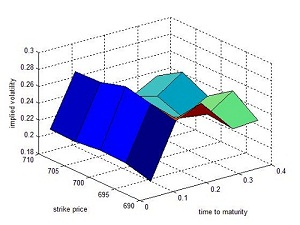
\includegraphics{volatility.jpg}
    \end{center}
    \caption{Implied Volatility Surface}
    \label{fig:master}
\end{figure}
\end{frame}

% New Section:Conclusion%
\section{Conclusion}
\begin{frame}
    \frametitle{Progress}
Have finished:
\begin{enumerate}
        \item Collected the Google's daily stock price data within recent two years
        \item Developed the code for generate implied volatility and generated the volatility surface
         \end{enumerate}
To do list: 
\begin{enumerate}
        \item Revise the Matlab code 
        \item Use Excel to apply three time series model to estimate historical volatility
        \item Compare the results and parametise the implied volitility surface
         \end{enumerate}
\end{frame}

\begin {frame}
\bibliographystyle{plain}
\nocite{*}
\bibliography{biblioMP}
\end {frame}
\end{document}
